\documentclass{article}
\usepackage[utf8]{inputenc}

% --- Language and Font Fix ---
\usepackage[english, vietnamese]{babel} 

\usepackage{amsmath, amsfonts, amssymb} % For mathematical equations and symbols
\usepackage{graphicx} % For including images
\usepackage{geometry} % For page layout
\geometry{a4paper, margin=1in} % Set page margins
\usepackage{tabularx} % For flexible table columns
\usepackage{enumitem} % For custom list environments
\usepackage{hyperref} % For clickable links in the table of contents
% --- Corrected Custom Commands for Vietnamese Text ---
\newcommand{\vietnameseuniversity}{\foreignlanguage{vietnamese}{ĐẠI HỌC BÁCH KHOA HÀ NỘI}}
\newcommand{\vietnameseschool}{\foreignlanguage{vietnamese}{TRƯỜNG CÔNG NGHỆ THÔNG TIN VÀ TRUYỀN THÔNG}}

\begin{document}

% --- Title Page/Header ---
\begin{titlepage}
    \centering
    \includegraphics[width=0.3\textwidth]{logo.png} 
    
    \vspace{1cm}
    
    {\Huge \vietnameseuniversity \par}
    \vspace{0.25cm}
    {\Large \vietnameseschool \par}
    
    \vspace{2cm}
    
    {\Huge \textbf{Report} \par}
    \vspace{0.5cm}
    {\Huge \textbf{Effects of superspreaders in spread of epidemic} \par}
    
    \vspace{2.5cm}

    \begin{tabular}{l l l}
        \textbf{Student name} & : & \foreignlanguage{vietnamese}{Phạm Anh Tú} \\
        \textbf{Student ID}   & : & 20225463 \\
        \textbf{Class}        & : & 157209 \\
        \textbf{Course}       & : & Mathematical Modeling \\
        \textbf{Course ID}    & : & IT4033E \\
        \textbf{Teacher}      & : & \foreignlanguage{vietnamese}{Bùi Quốc Trung} \\
    \end{tabular}
    
    \vfill 
    
    {\large \textit{\foreignlanguage{vietnamese}{Hà Nội}, 24th May 2025} \par}
\end{titlepage}

\clearpage

% --- Table of Contents ---
\tableofcontents
\clearpage

% --- I. INTRODUCTION ---
\section{INTRODUCTION}
\label{sec:introduction}
Analyzing infectious disease dynamics is crucial for public health, enabling outbreak predictions and the evaluation of control measures. Traditional epidemiological models often simplify population characteristics, assuming homogeneity in factors like infectiousness and contact rates. However, real-world epidemics are frequently characterized by significant heterogeneity, where a small number of individuals contribute disproportionately to transmission. These individuals, known as "superspreaders," can drive "superspreading events" (SSEs) that dramatically accelerate and widen the scope of an outbreak. The 2003 SARS (Severe Acute Respiratory Syndrome) epidemic prominently featured such events, highlighting the need for models that can account for this phenomenon.

The reference paper, "Effects of superspreaders in spread of epidemic" by Ryo Fujie and Takashi Odagaki (2007), directly addresses this challenge. It aims to investigate the impact of superspreaders by proposing and simulating two distinct mechanisms for superspreading behavior within a spatial Susceptible-Infected-Recovered (SIR) framework. This report will review the modeling approach, mathematical formulation, simulation algorithm, and key conclusions presented by Fujie and Odagaki. Furthermore, it will discuss the model's sensitivity and robustness, potentially drawing insights from a Python implementation of these models.

% --- II. MODELING APPROACH ---
\section{MODELING APPROACH}
\label{sec:modeling_approach}
Fujie and Odagaki (2007) started from a standard Susceptible-Infected-Recovered (SIR) model analysis, but with some significant additions to allow for the complexities of superspreading.

Their key modeling elements are :
\begin{itemize}[leftmargin=*, align=left]
    \item \textbf{Spatial Structure}: The subjects (N total) are spread in a continuous two-dimensional space of size L x L with fixed positions. Periodic boundary conditions are implemented to minimize edge effects. This spatial structure allows distance-dependent interactions to be specified, beyond the mean-field assumptions of non-spatial compartmental models.
    \item \textbf{Distance-Dependent Infection Probability (\(w(r)\))}: The infection probability of a susceptible person by an infected person is a function of the Euclidean distance \(r\) separating the two. This captures the intuitive notion that contacts between people who are in close proximity to each other are more likely to lead to infection.
    \item \textbf{Two Distinct Superspreader Models}: To explore other underlying mechanisms for superspreading, the authors proposed two hypotheses, which were implemented as two alternate models for superspreader individuals (who comprise a fraction \(\lambda\) of the population) :
    \begin{itemize}
        \item \textbf{Strong Infectiousness Model}: Superspreaders simply have a higher probability of infecting others within the same interaction radius (cutoff distance \(r_0\)) as normal individuals.
        \item \textbf{Hub Model}: Superspreaders are characterized as having a vastly larger interaction range than normal people. This represents individuals with more social contacts or opportunities to transmit the disease over long distances, even if their intrinsic infectiousness profile within that range is identical to normal people.
    \end{itemize}
\end{itemize}
This modeling approach was chosen to better approximate the spread of epidemics in the real world. The SIR model needed generalization to represent the differential impact of superspreaders. While more complex network models exist, the authors chose a "simplified model" that still incorporated essential elements like spatiality and distance to directly investigate superspreader mechanisms. Their ultimate goal was to see if these simplified models could reproduce observed phenomena in the SARS epidemic.

% --- III. MATHEMATICAL MODELING ---
\section{MATHEMATICAL MODELING}
\label{sec:mathematical_modeling}
N individuals are randomly placed (except for the initial infector) with fixed positions \(p_i\) in an L x L continuous space with periodic boundary conditions. Each individual \(i\) can be in one of three states at a given time step \(t\): susceptible (S), infected (I), or recovered (R). Initially, there are N - 1 susceptible individuals and 1 infected. Infected individuals can turn to recovered state with probability \(\gamma\). Initially, there are exactly \(\lfloor \lambda N \rfloor\) superspreaders.

Since we are using periodic boundary conditions, the distance of two individuals \(i\) and \(j\) is given by :
\[
r = d(i, j) = \sqrt{\sum_k \min(|p_{i, k} - p_{j, k}|, L - |p_{i, k} - p_{j, k}|)^2}
\]
The probability of an infected individual at \(p_j\) infecting a susceptible individual at \(p_i\) at distance \(r\) within one Monte Carlo step is :
\[
w(r) = w_0 \cdot \left(1 - \frac{r}{r_0}\right)^\alpha \quad \text{for } 0 < r \le r_0
\]
\[
w(r) = 0 \quad \text{for } r > r_0
\]
In the strong infectious model, \(\alpha\) is equal to 0 for superspreaders, meaning a susceptible individual in range \(r_0\) with an infected individual is guaranteed to be infected. For normal individuals, \(\alpha\) is set to 2.

In the hub model, superspreaders make more contact with other people, so their cutoff distance is longer. Specifically, a superspreader cutoff distance is \(r_n = \sqrt{6} \cdot r_0\).
\[
w(r) = w_0 \cdot \left(1 - \frac{r}{r_n}\right)^2 \quad \text{for } 0 < r \le r_n
\]
\[
w(r) = 0 \quad \text{for } r > r_n
\]
where \(r_n = \sqrt{6} \cdot r_0\).

% --- IV. SOLVING ALGORITHM ---
\section{SOLVING ALGORITHM}
\label{sec:solving_algorithm}
The solving algorithm used in the reference paper is Monte Carlo simulation. The simulation was run 1000 times with different initial positions, and the average of some quantities was logged. They used the following parameter settings :
\begin{itemize}
    \item \(N\) in range 150 to 900
    \item \(L = 10r_0\)
    \item \(w_0 = 1\)
    \item \(\gamma = 1\)
\end{itemize}
In our experiments, we lower the number of simulation runs to 100 for some experiments and modify our parameter settings to better suit our computational resources :
\begin{itemize}
    \item \(N = 200\)
    \item \(L = \sqrt{\frac{N \cdot \pi \cdot r_0^2}{\text{density}}}\)
    \item Density in range 0 to 25
\end{itemize}

% --- V. RESULTS ---
\section{RESULTS}
\label{sec:results}
\subsection{Percolation probability}
\label{sec:results_percolation}
The original paper defined percolation as the event when the infection started at the bottom of the system reaches on the top of it. The percolation probability is then defined as the fraction of runs in which percolation occurs. The paper did not provide definitions of "bottom" and "top" of the system, so we assume that bottom is the state with only one infected individual and top is the state where all individuals are infected. 

Replicating the experiment with our parameter settings, we achieve similar results. Figure \ref{fig:percolation_probability} shows the function of percolation probability on several values of \(\lambda\) (superspreader fraction) for both Strong Infectiousness and Hub Models. In the case of no superspreader (\(\lambda = 0\)), the infection rarely reach the top state. As \(\lambda\) increases, the percolation probability also rapidly increases at lower density values.

\begin{figure}[!htbp]
    \centering
    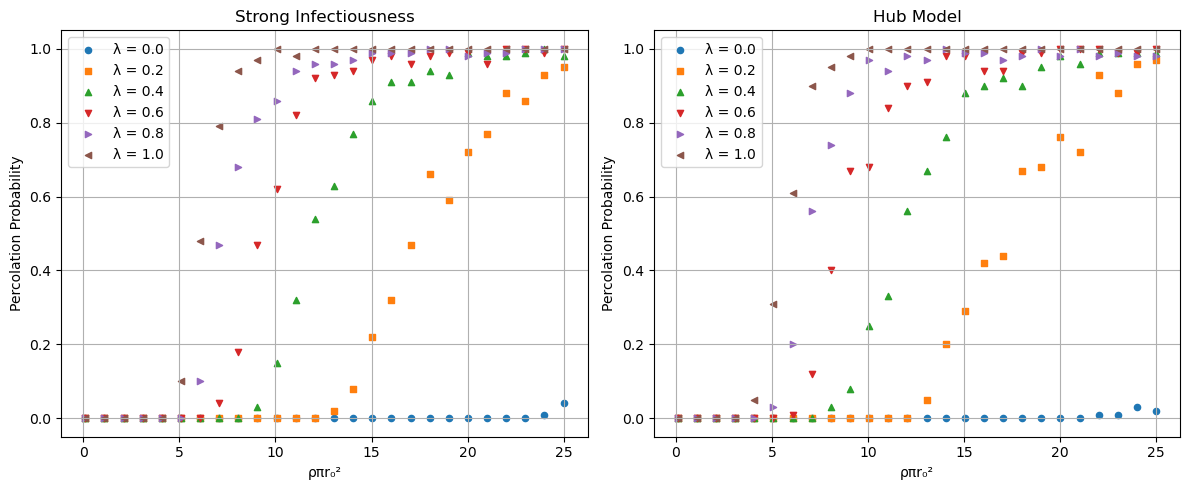
\includegraphics[width=0.9\textwidth]{fig/percolation.png} 
    \caption{Percolation probability as a function of \(\rho\pi r_0^2\) for both Strong Infectiousness and Hub Models, demonstrating the effect of different superspreader fractions \(\lambda\).}
    \label{fig:percolation_probability}
\end{figure}

\subsection{Propagation velocity}
\label{sec:results_propagation_velocity}
The paper defined the velocity of propagation as the velocity of front line. Let \(r_f\) be the distance between the initial infected individual and the furthest infected individual. The velocity is then defined as:
\[
\frac{r_f}{r_0 \cdot t}
\]
where \(t\) is the time step when the furthest infected individual is reached. We calculate the average propagation velocity as the average of velocities over all runs. As shown in Figure \ref{fig:propagation_speed}, the propagation velocity of the hub model is consistently larger than that of the strong infectiousness model. 
\begin{figure}[!htbp]
    \centering
    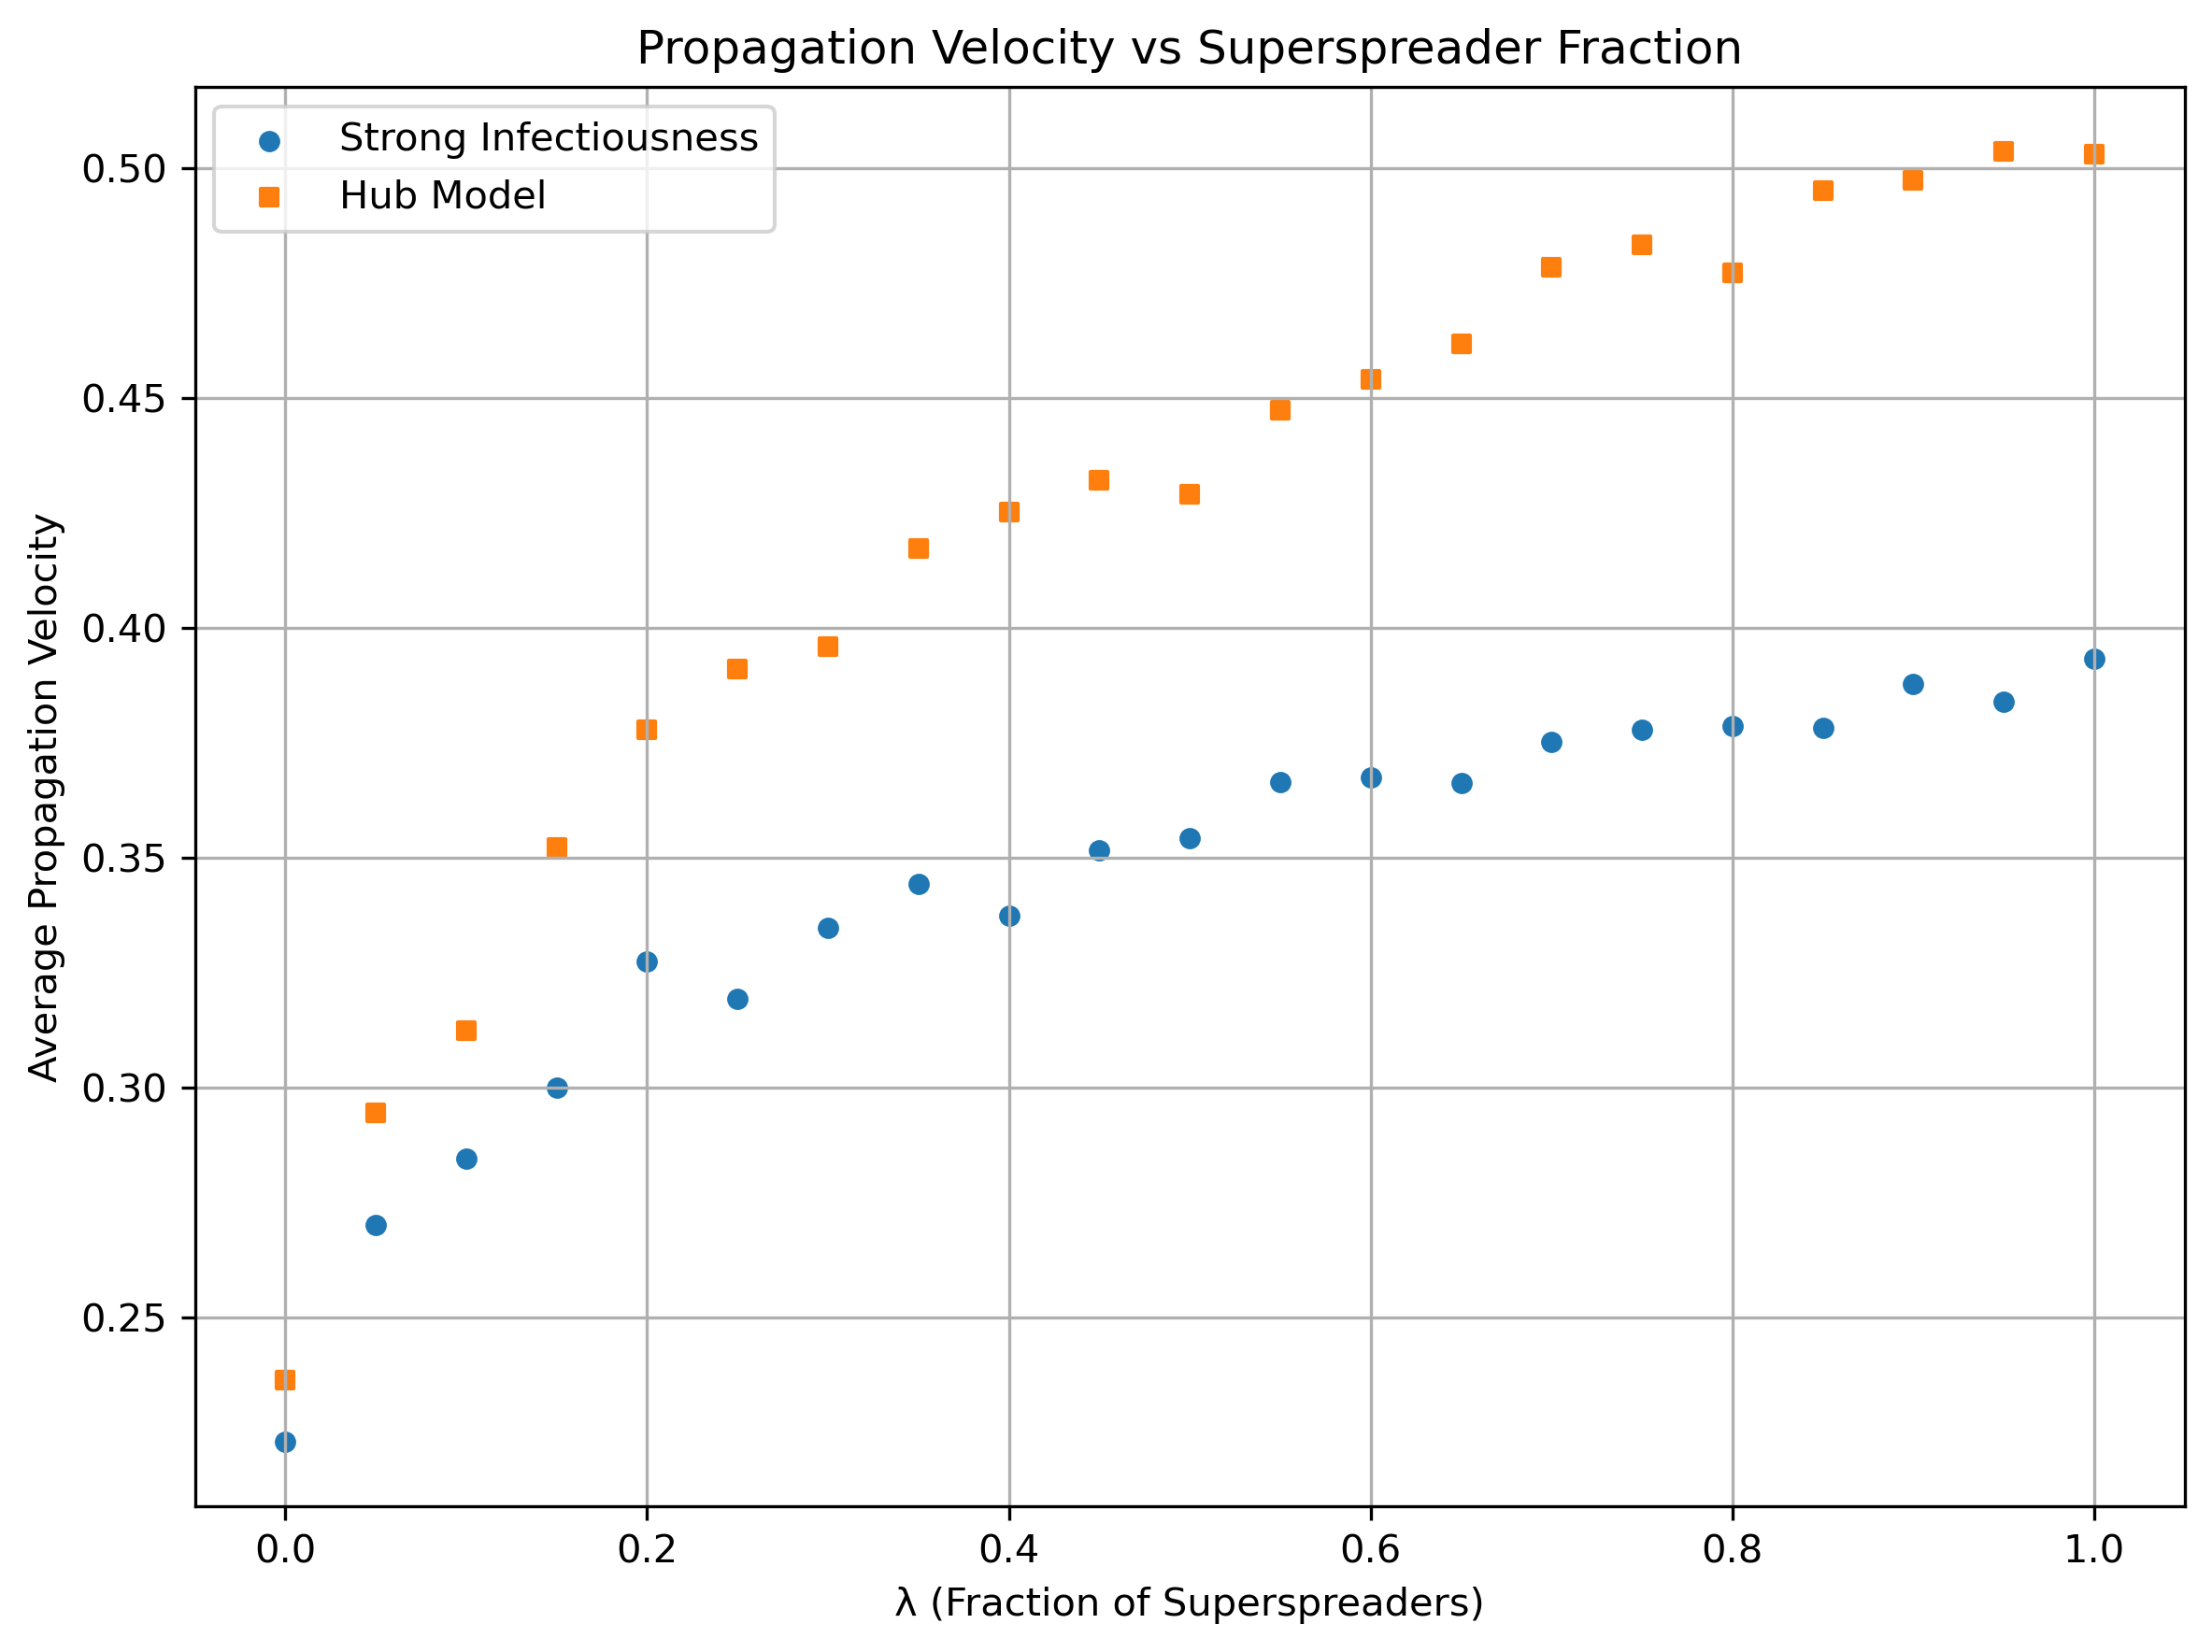
\includegraphics[width=0.8\textwidth]{fig/velocity.png} 
    \caption{Average Propagation Velocity versus the fraction of superspreaders (\(\lambda\)) for both Strong Infectiousness and Hub Models.}
    \label{fig:propagation_speed}
\end{figure}

\subsection{Infection Distribution}
\label{sec:results_infection_distribution}
We visualize each step of the simulation to see how the infected individuals are distributed on the LxL space over time. Figures \ref{fig:side_by_side_snapshots_1}, \ref{fig:side_by_side_snapshots_2}, and \ref{fig:side_by_side_snapshots_3} compare the two models in each time step for a short simulation. A common trend we found is that infected individuals in the hub model are more spread out than in the strong infectious model. However, strong infectious model does prolong the epidemic longer thanks to the guaranteed infectiousness, which we will investigate further in the next section.

\begin{figure}[!htbp]
    \centering
    \begin{tabular}{cc}
        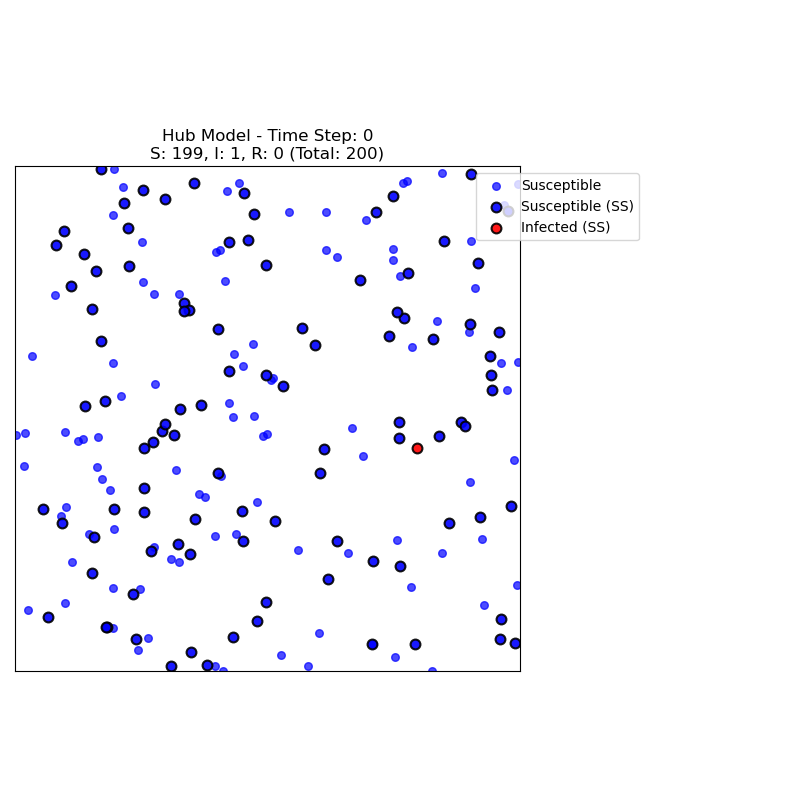
\includegraphics[width=0.4\textwidth]{fig/sir_hub_step_0.png} &
        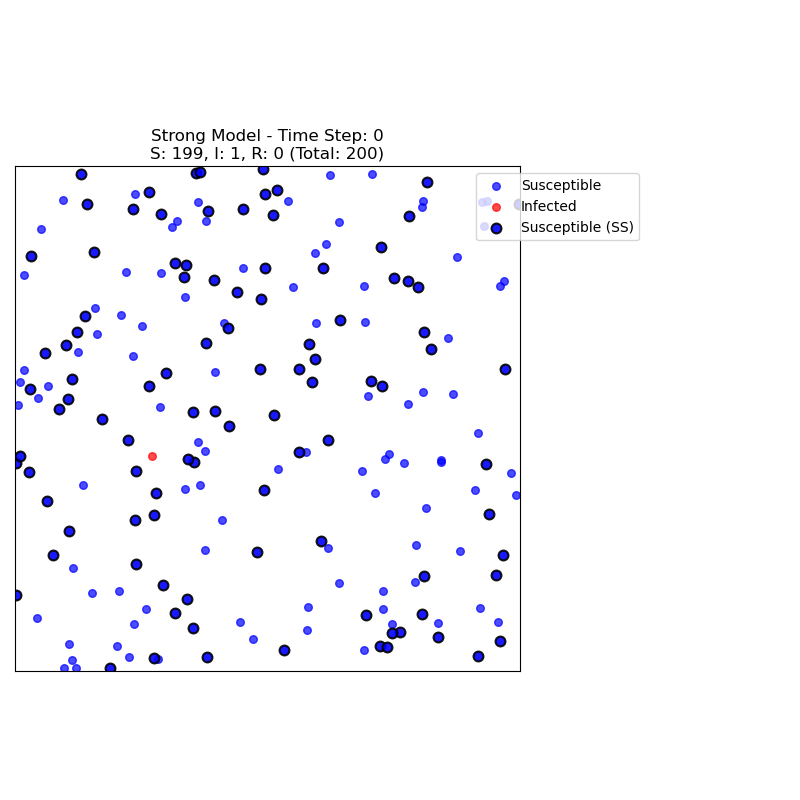
\includegraphics[width=0.4\textwidth]{fig/sir_strong_step_0.png} \\
        Hub Model (Step 0) & Strong Infectiousness Model (Step 0) \\
        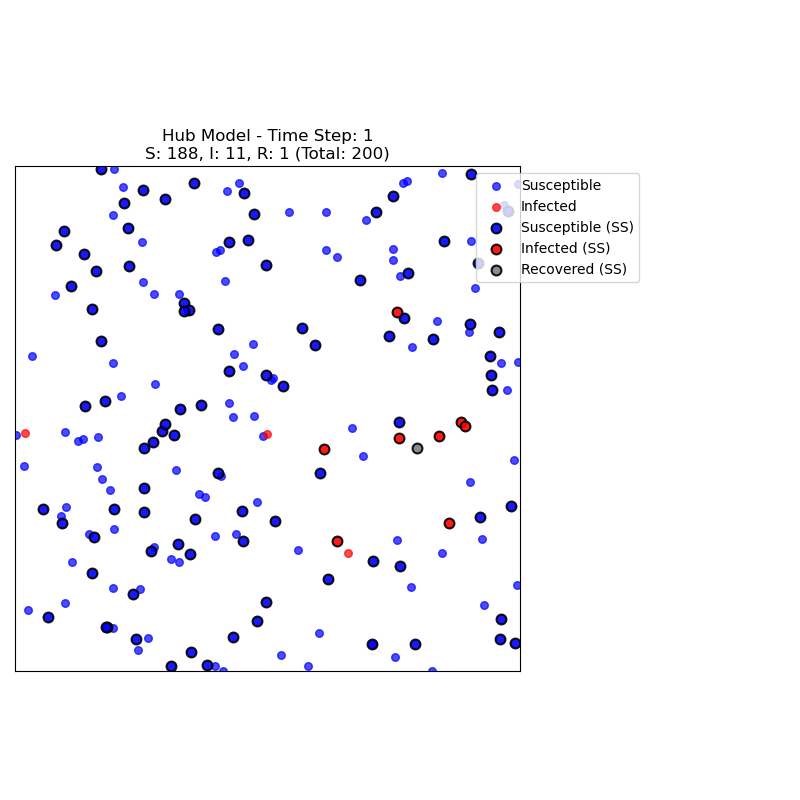
\includegraphics[width=0.4\textwidth]{fig/sir_hub_step_1.png} &
        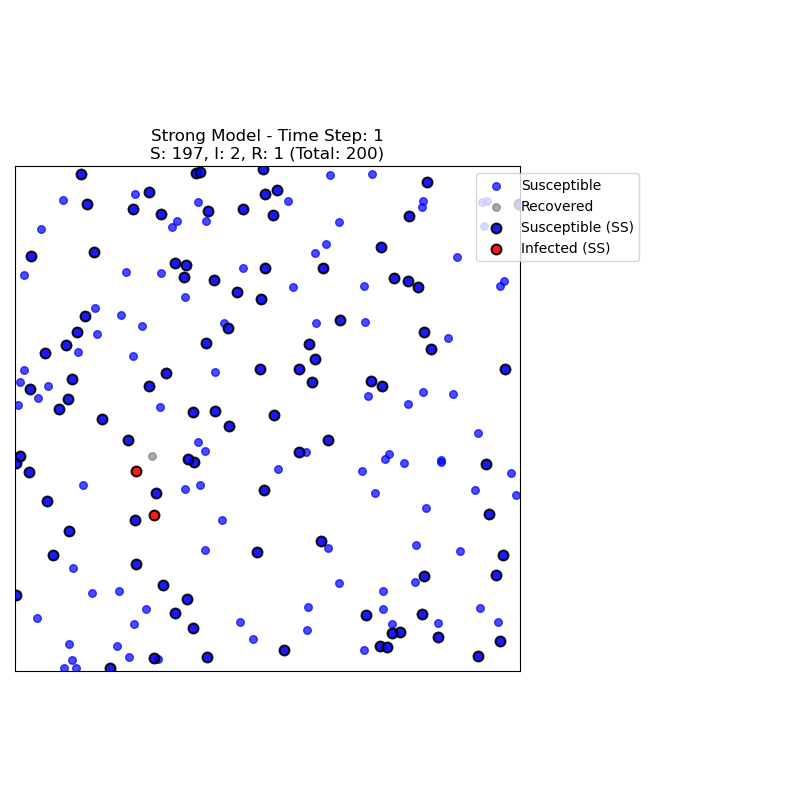
\includegraphics[width=0.4\textwidth]{fig/sir_strong_step_1.png} \\
        Hub Model (Step 1) & Strong Infectiousness Model (Step 1) \\
    \end{tabular}
    \caption{Side-by-side snapshots of the Hub Model (left) and Strong Infectiousness Model (right) at time steps 0 and 1. Blue: Susceptible, Red: Infected, Grey: Recovered. Superspreaders are outlined in black.}
    \label{fig:side_by_side_snapshots_1}
\end{figure}

\begin{figure}[!htbp]
    \centering
    \begin{tabular}{cc}
        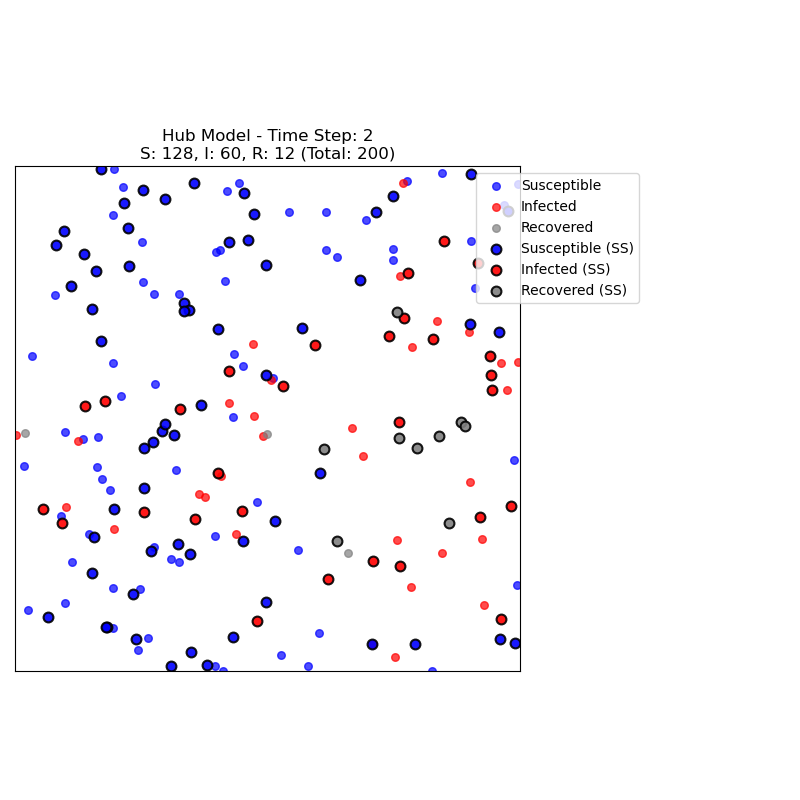
\includegraphics[width=0.4\textwidth]{fig/sir_hub_step_2.png} &
        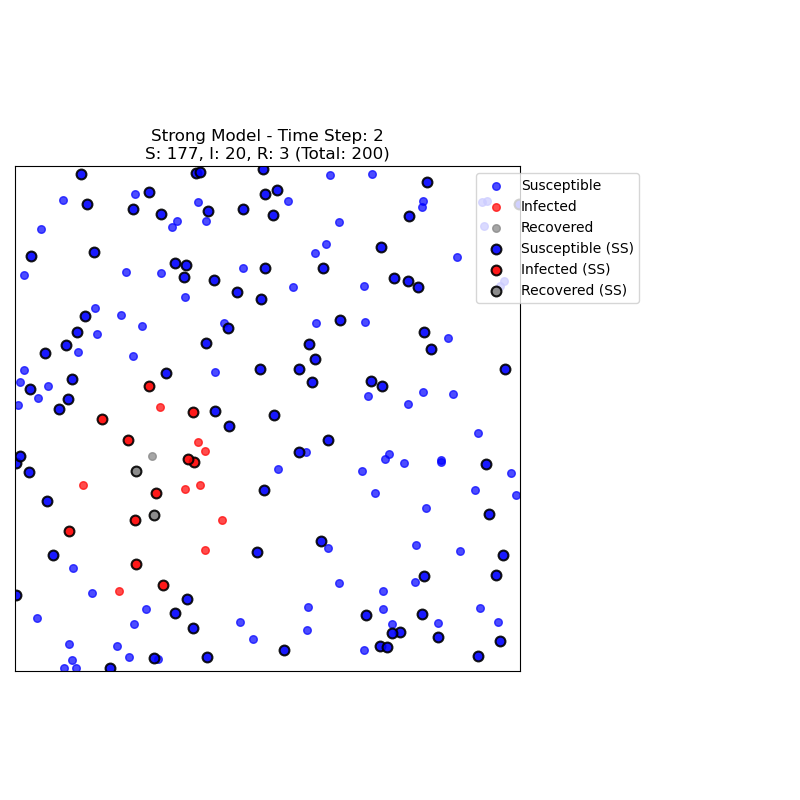
\includegraphics[width=0.4\textwidth]{fig/sir_strong_step_2.png} \\
        Hub Model (Step 2) & Strong Infectiousness Model (Step 2) \\
        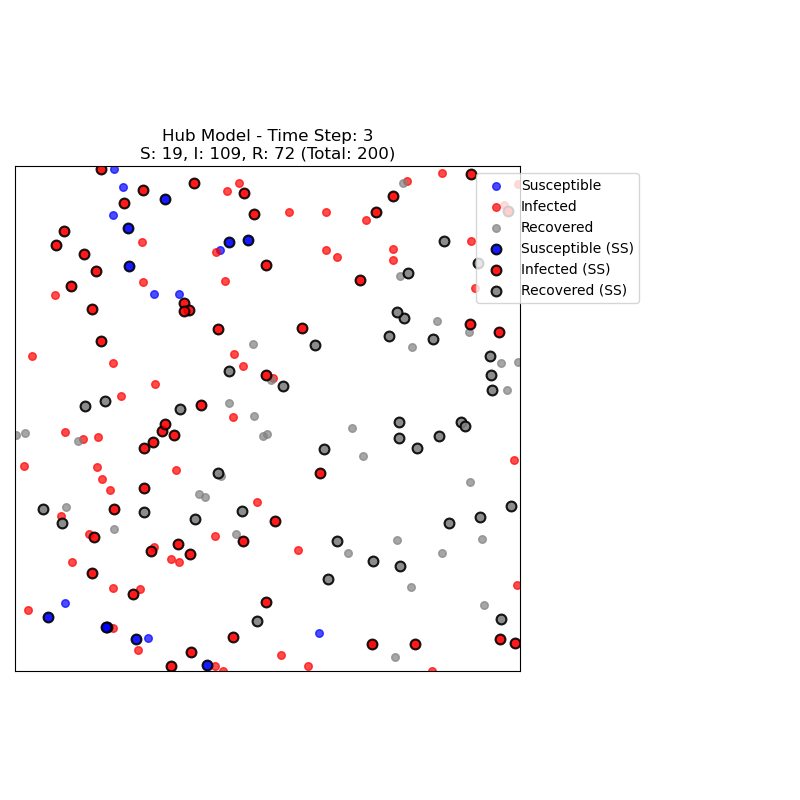
\includegraphics[width=0.4\textwidth]{fig/sir_hub_step_3.png} &
        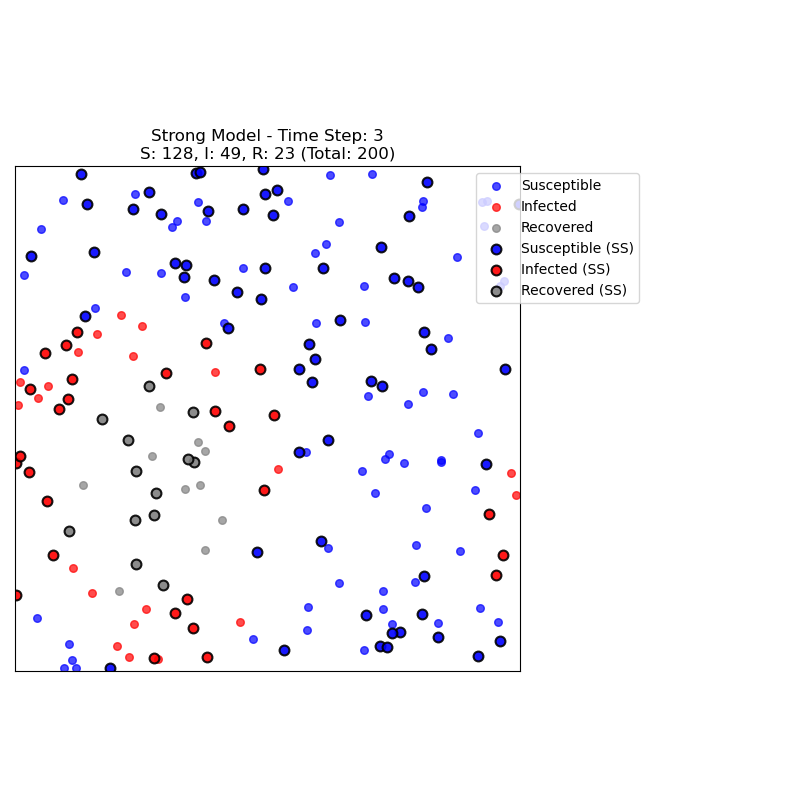
\includegraphics[width=0.4\textwidth]{fig/sir_strong_step_3.png} \\
        Hub Model (Step 3) & Strong Infectiousness Model (Step 3) \\
        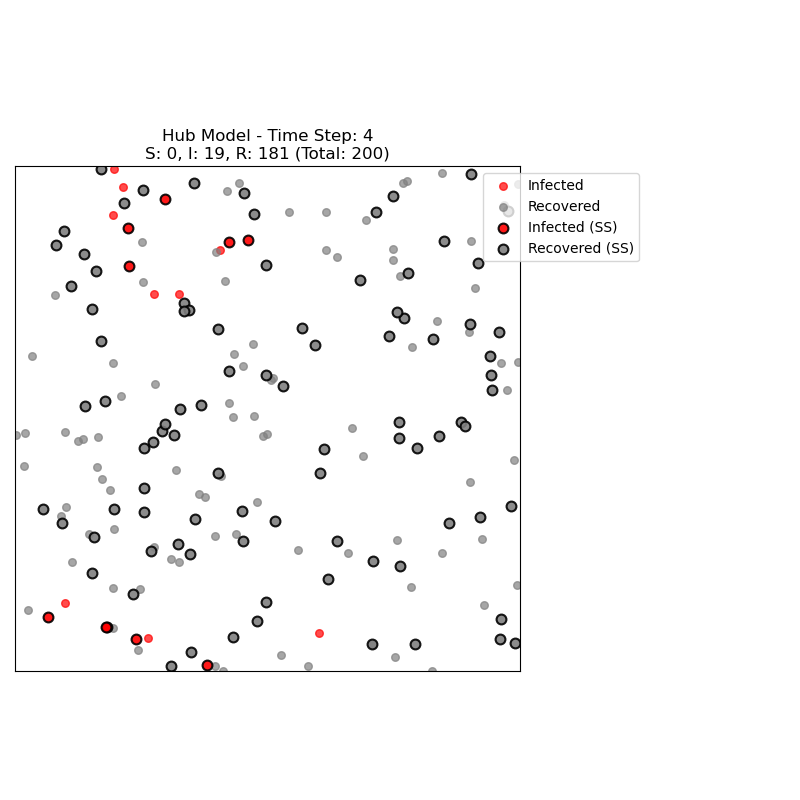
\includegraphics[width=0.4\textwidth]{fig/sir_hub_step_4.png} &
        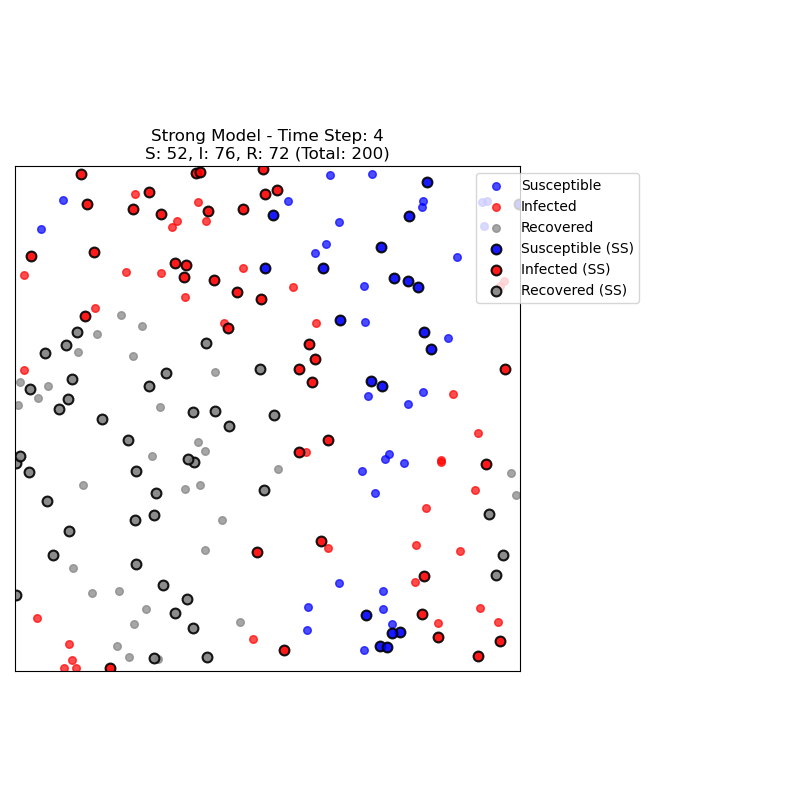
\includegraphics[width=0.4\textwidth]{fig/sir_strong_step_4.png} \\
        Hub Model (Step 4) & Strong Infectiousness Model (Step 4) \\
    \end{tabular}
    \caption{Side-by-side snapshots of the Hub Model (left) and Strong Infectiousness Model (right) at time steps 2 and 4. Blue: Susceptible, Red: Infected, Grey: Recovered. Superspreaders are outlined in black.}
    \label{fig:side_by_side_snapshots_2}
\end{figure}

\begin{figure}[!htbp]
    \centering
    \begin{tabular}{cc}
        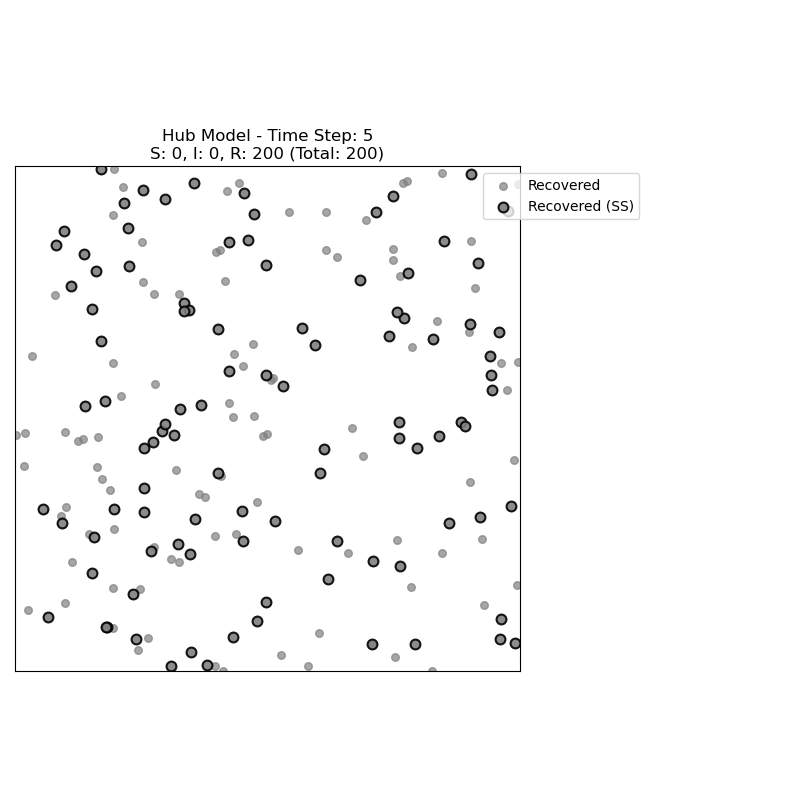
\includegraphics[width=0.4\textwidth]{fig/sir_hub_step_5.png} &
        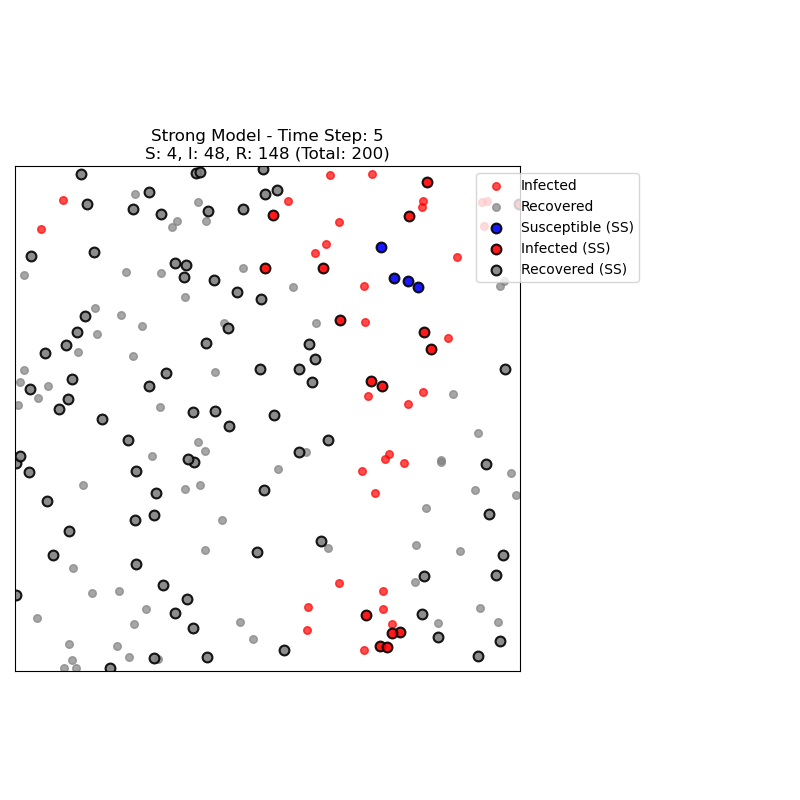
\includegraphics[width=0.4\textwidth]{fig/sir_strong_step_5.png} \\
        Hub Model (Step 5) & Strong Infectiousness Model (Step 5) \\
        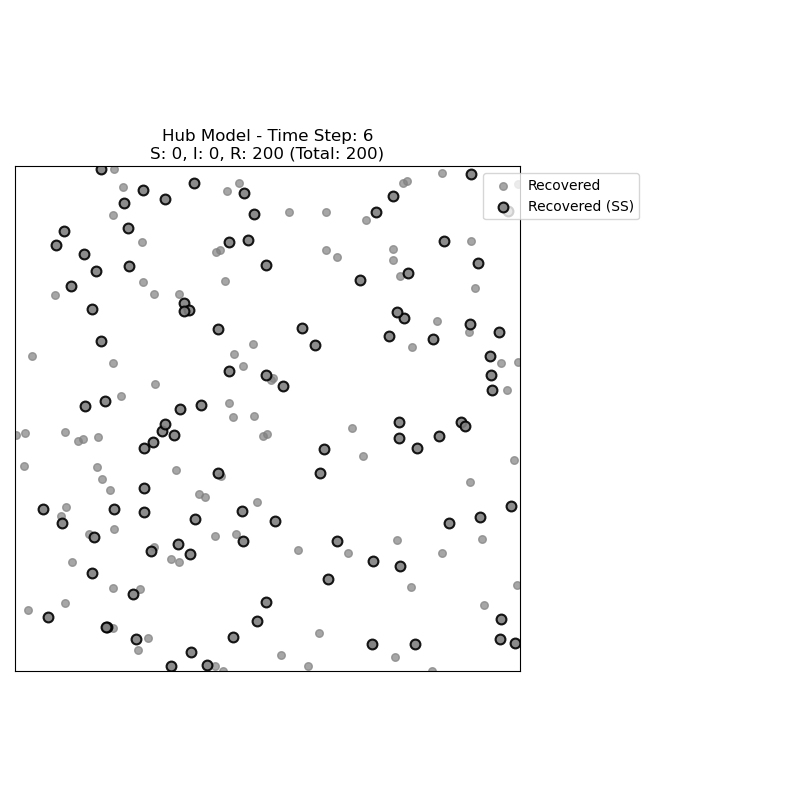
\includegraphics[width=0.4\textwidth]{fig/sir_hub_step_6.png} &
        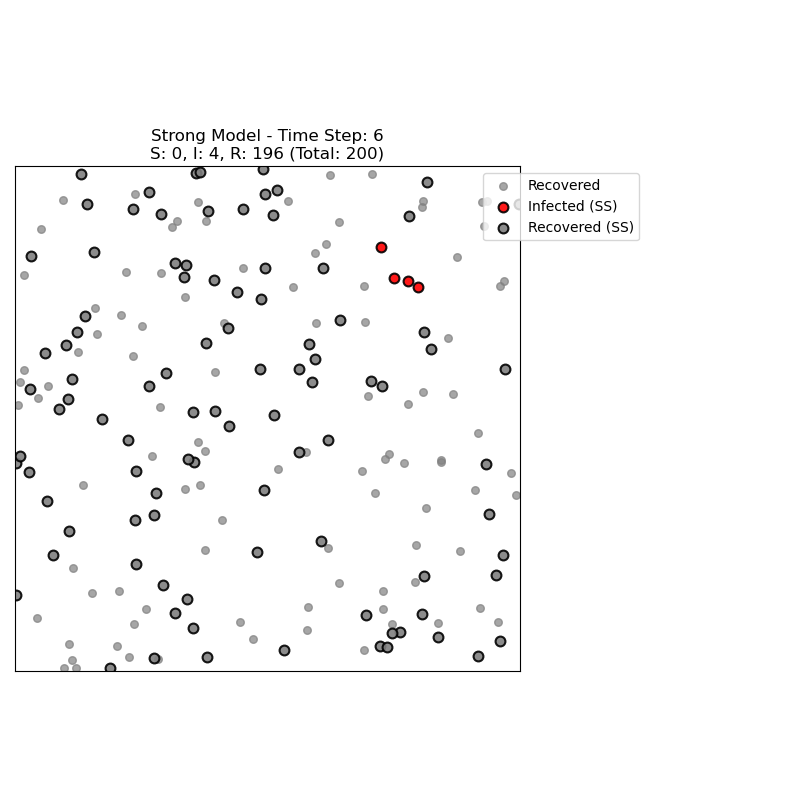
\includegraphics[width=0.4\textwidth]{fig/sir_strong_step_6.png} \\
        Hub Model (Step 6) & Strong Infectiousness Model (Step 6) \\
    \end{tabular}
    \caption{Side-by-side snapshots of the Hub Model (left) and Strong Infectiousness Model (right) at time steps 5 to 6. Blue: Susceptible, Red: Infected, Grey: Recovered. Superspreaders are outlined in black.}
    \label{fig:side_by_side_snapshots_3}
\end{figure}

\subsection{Epidemic curves}
\label{sec:results_epidemic_curves}
We follow the original paper to plot the epidemic curves, which show the number of infected individuals over time. The curves are averaged over 100 runs for each model with a simple parameter sweep for \(\lambda \). Figure \ref{fig:epidemic_curve} shows the epidemic curves for both models compared to the SARS data from 2003. The strong infectiousness model shows a longer duration of infection, while the hub model leads to a faster spread but shorter duration. For \(\lambda = 0.2\), the Hub Model's curve is similar to the SARS data, indicating that a small fraction of superspreaders can significantly impact the epidemic dynamics.
\begin{figure}[!htbp]
    \centering
    % \begin{tabular}{cc} % Not needed for a single image
        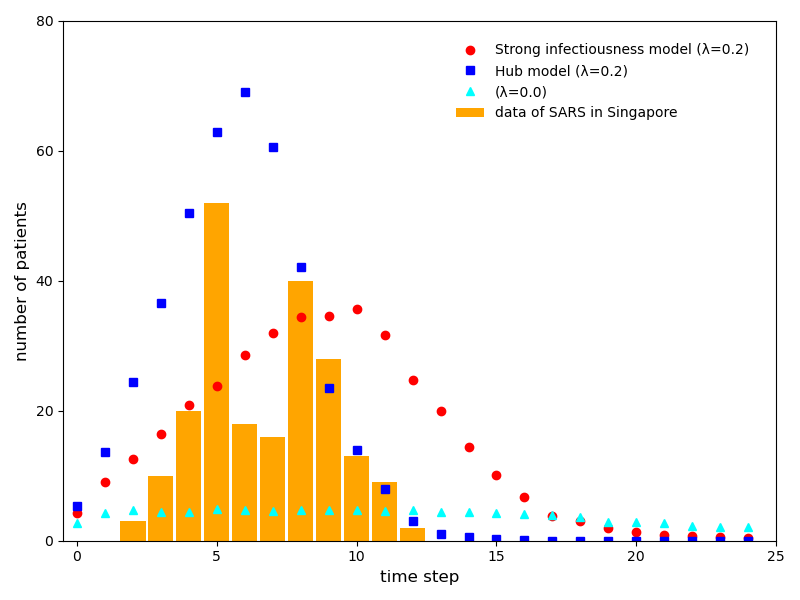
\includegraphics[width=0.7\textwidth]{fig/epidemic_curve.png}
    % \end{tabular}
    \caption{Number of patients of both models compare to SARS data from 2003}
    \label{fig:epidemic_curve}
\end{figure}

\section{Sensitivity Analysis}
\label{sec:sensitivity_analysis}

Sensitivity analysis is crucial for understanding the robustness of a model's predictions and identifying which parameters or assumptions most significantly influence its outcomes. In this study, while not exhaustively exploring the entire parameter space of the original Fujie \& Odagaki (2007) paper due to computational resource constraints (e.g., N=200, 100 simulation runs), several key sensitivities can be discussed based on our experiments.

\subsection{Sensitivity to Superspreader Fraction ($\lambda$)}
\label{sec:sensitivity_lambda}

The fraction of superspreaders ($\lambda$) in the population is arguably one of the most critical parameters investigated, and our results consistently demonstrate the model's high sensitivity to its value.

\begin{itemize}
    \item \textbf{Percolation Probability (Figure \ref{fig:percolation_probability}):} 
    As observed in Section \ref{sec:results_percolation}, increasing $\lambda$ dramatically impacts the percolation probability. For both the Strong Infectiousness and Hub models, a higher fraction of superspreaders leads to the epidemic percolating (spreading system-wide) at significantly lower overall population densities ($\rho\pi r_0^2$). This indicates that even a small proportion of superspreaders can greatly enhance the disease's ability to invade and persist in a population. The transition from non-percolation to percolation also becomes sharper with increasing $\lambda$.

    \item \textbf{Propagation Velocity (Figure \ref{fig:propagation_speed}):}
    Section \ref{sec:results_propagation_velocity} and Figure \ref{fig:propagation_speed} clearly show that the average propagation velocity of the epidemic front is highly sensitive to $\lambda$. For both models, velocity increases with $\lambda$. This is intuitive, as superspreaders, by either enhanced infectivity or wider reach, accelerate the transmission process.

    \item \textbf{Epidemic Curves (Figure \ref{fig:epidemic_curve} and Figure \ref{fig:sensitivity_analysis}):}
    The shape and scale of the epidemic curve (number of newly infected individuals over time) are profoundly affected by $\lambda$. As seen in Figure \ref{fig:epidemic_curve} when comparing $\lambda=0.0$ (no superspreaders) with $\lambda=0.2$ for the Hub Model, the presence of superspreaders leads to a faster rise and a higher peak. Figure \ref{fig:sensitivity_analysis} further illustrates this by demonstrating how increasing $\lambda$ results in epidemics that are more explosive (higher, earlier peaks) but potentially of shorter duration as the susceptible pool is depleted more rapidly, which are present in both models.
\end{itemize}

\begin{figure}[!htbp]
    \centering
    % \begin{tabular}{cc} % Not needed for a single image
        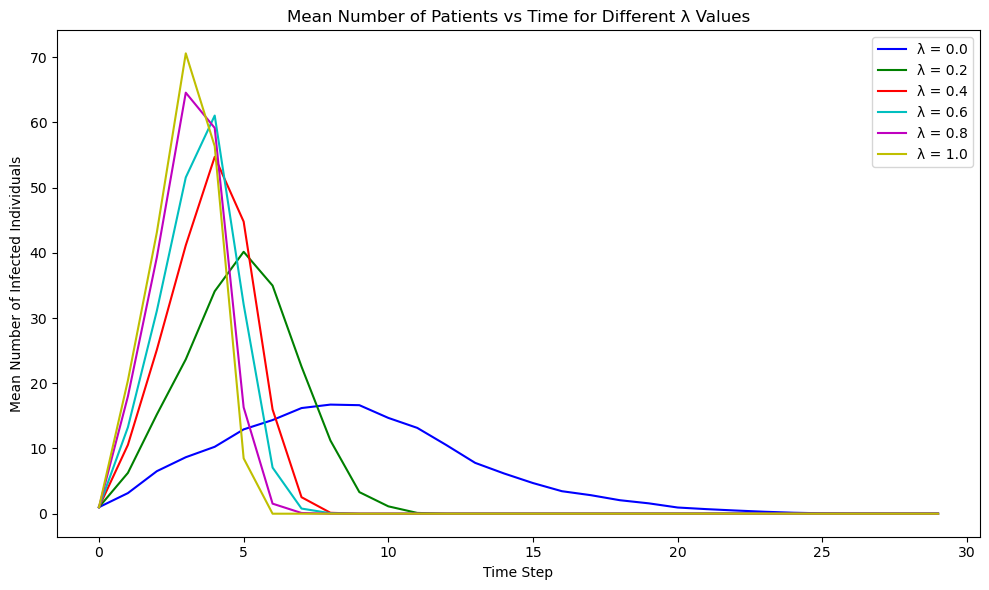
\includegraphics[width=0.7\textwidth]{fig/sensitivity_analysis.png}
    % \end{tabular}
    \caption{Sensitivity analysis of the number of infected individuals for Strong Infectious model on \(\lambda\). The results are the average of 1000 simulations}
    \label{fig:sensitivity_analysis}
\end{figure}


\subsection{Structural Sensitivity: Choice of Superspreader Model}
\label{sec:sensitivity_structural}

The choice between the Strong Infectiousness model and the Hub model represents a structural sensitivity analysis, as it tests different underlying mechanisms for superspreading.

\begin{itemize}
    \item \textbf{Propagation Velocity (Figure \ref{fig:propagation_speed}):}
    A key finding, consistent with the original paper, is that the Hub model consistently yields significantly higher propagation velocities than the Strong Infectiousness model for any given $\lambda > 0$.

    \item \textbf{Infection Distribution (Figures \ref{fig:side_by_side_snapshots_1}, \ref{fig:side_by_side_snapshots_2}, and \ref{fig:side_by_side_snapshots_3}):}
    The qualitative snapshots of infection distribution (Section \ref{sec:results_infection_distribution}) illustrate differences in spatial patterns. The Hub model tends to show a more dispersed pattern of infection due to the longer reach of its superspreaders. In contrast, the Strong Infectiousness model, with its guaranteed infection probability within $r_0$ for superspreaders, can lead to more intense local clusters and, as noted in our observations, potentially prolong the epidemic if susceptible individuals are continuously available within that range.

    \item \textbf{Epidemic Curves (Figure \ref{fig:epidemic_curve}):}
    As discussed in Section \ref{sec:results_epidemic_curves}, the two models produce different epidemic curve profiles. Our observations suggest the Strong Infectiousness model tends towards a longer duration of infection. The Hub model, while leading to faster spread, may exhibit a shorter overall duration. The observation that the Hub model with $\lambda=0.2$ (as shown in Figure \ref{fig:epidemic_curve}) better approximates the real-world SARS data underscores the model's sensitivity to this structural assumption and its relevance in capturing real epidemic features.
\end{itemize}

\subsection{Sensitivity to Other Model Parameters and Assumptions (Qualitative Discussion)}
\label{sec:sensitivity_other}

While our experiments focused on $\lambda$, $\rho\pi r_0^2$, and the choice of superspreader model, the overall model behavior is also sensitive to other parameters and assumptions:

\begin{itemize}
    \item \textbf{Fixed Parameters ($w_0, \gamma, \alpha$):} In our simulations, and largely in the original paper for the main results, $w_0=1$, $\gamma=1$, and $\alpha=2$ (for normal/Hub) were fixed. Changes to $w_0$ (base infectivity), $\gamma$ (recovery rate, inversely related to infectious period), or $\alpha$ (decay of infection with distance) would quantitatively alter all results. For instance, a lower $\gamma$ would prolong the infectious period, likely leading to larger epidemics.
    \item \textbf{Population Size ($N$) and System Size ($L$):} We used $N=200$, differing from the broader range in the original paper. While $\rho\pi r_0^2$ normalizes for density, very small $N$ can lead to greater stochastic fluctuations and potentially make percolation thresholds less distinct. $L$ is determined by $N$, $r_0$, and the target density.
    \item \textbf{Number of Simulation Runs:} We used 100 runs for averaging, compared to 1000 in the original paper. While sufficient to observe trends, a higher number of runs would provide smoother curves and more statistically robust quantitative estimates, especially near critical thresholds.
    \item \textbf{Initial Conditions:} The placement of the initial infector and the number of initial infectors can affect the early dynamics and overall outcomes.
    \item \textbf{Fixed Agent Positions:} A core assumption is that individuals do not move. Introducing mobility would fundamentally change the contact structure and likely alter all observed dynamics. The current model's conclusions are robust only within this static framework.
\end{itemize}

\subsection{Robustness of Observed Trends in Our Study}
\label{sec:sensitivity_robustness}

Despite the reduced computational scope compared to the original paper (e.g., $N=200$, 100 simulation runs for averaging), the qualitative trends observed in our experiments appear robust and are consistent with the findings of Fujie \& Odagaki (2007). For example, the effect of increasing $\lambda$ in lowering percolation thresholds and increasing propagation speed, as well as the distinct behaviors of the Hub versus Strong Infectiousness models, were clearly replicated. This suggests that the fundamental impacts of introducing superspreaders through these mechanisms are observable even with moderately sized systems. The visual similarity of our Hub model's epidemic curve (with $\lambda=0.2$) to the SARS data in Figure \ref{fig:epidemic_curve} further supports the relevance of this particular model structure.

\section{Conclusion}
In conclusion, this report reimplements the modeling of Fujie & Odagaki (2007) and replicate some key results. We also discuss about the sensitivity and robustness of our model to important parameters and show that the model exhibits significant sensitivity to the fraction of superspreaders and the chosen mechanism of superspreading. Further investigation could more deeply explore the quantitative impact of parameters such as γ and α, and the structural implications of introducing factors like agent mobility.
\section{Reference}
\begin{thebibliography}{9}
\bibitem{fujie2007}
Ryo Fujie and Takashi Odagaki,
\textit{Effects of superspreaders in spread of epidemic},
Physica A: Statistical Mechanics and its Applications, Volume 373, 2007, Pages 445-454.
\url{https://www.sciencedirect.com/science/article/pii/S0378437106008703}
\end{thebibliography}
\end{document}